\documentclass{csmathnotes}
\usepackage{biblatex}

\udc{519.832.2}

\title{Некоторые стратегии для «Игры в подстановки»}

\author{Гладков Артемий Николаевич}
\affiliation{Ярославский государственный университет им. П.Г. Демидова}
\email{gladkov.art76@gmail.com} % Email должен быть тем, которым реально пользуется автор!

\author{Смирнов Александр Валерьевич}
\affiliation{Ярославский государственный университет им. П.Г. Демидова}
\email{alexander_sm@mail.ru}


% Если авторов или руководителей больше одного, продублируйте и заполните соответствующий блок

\newtheorem{algoritm}{Алгоритм} 
\newtheorem{definition}{Определение} 
\newtheorem{weight}{Распределение весов}
\newtheorem{metric}{Метрика}
\newtheorem{statement}{Утверждение}


\addbibresource{Gladkov.bib}

\newcommand{\R}{\mathbb{R}}

\begin{document}

\maketitle

\begin{abstract}
В работе рассматривается игра, основанная на контекстно-свободной грамматике, под названием <<Игра в подстановки>>. Приводится описание чистых и смешанных стратегий, проводится их сравнительный анализ. 

\keywords{стратегия, сравнительный анализ, контекстно-свободная грамматика, чистая стратегия, смешанная стратегия}
\end{abstract}

\section*{Введение}

Будем рассматривать антагонистическую контекстно-свободную игру, в которой два игрока стремятся максимизировать свой выигрыш, получая как можно больше сентенций как можно большей суммарной длины, строя выводы в выбранной контекстно-свободной грамматике. В игру вводится элемент случайности: доступные продукции определяются броском двух кубиков; кроме них также можно использовать продукции, находящиеся в банке продукций. Мы разработаем стратегии для игрока-компьютера, которые будут основаны на анализе продукций грамматики и имеющихся текущих выводов.

Отметим, что близкие задачи рассматриваются в~\cite{Schuster:2017}. В~этой диссертации исследуется целый класс контекстно-свободных игр. В самом простом варианте первому игроку доступен выбор нетерминала, который необходимо заменить, а второй игрок выбирает какую последовательность символов, соответствующую правилам данной контекстно-свободной грамматики, вставить. Вопрос состоит в том, имеет ли первый игрок выигрышную стратегию, если его задача получить определённую сентенциальную форму или одну из сентенциальных форм из определённого множества. В работе рассматривается вопрос разрешимости а также проводится анализ сложности этой задачи при разных ограничениях и дополнительных условиях. Тем не менее, постановки всех задач из~\cite{Schuster:2017} так или иначе отличаются от~нашей.

\section*{Постановка задачи}

%\begin{definition}[см. пособие~\cite{Sokolov:2014}]
%	\emph{Грамматикой} $G$ называется упорядоченная четвёрка $G=(N,T,S,P)$, где 
%	\begin{itemize}
%		\item$N$ "--- конечное множество \emph{нетерминальных символов};
%		
%		\item$T$ "--- конечное множество \emph{терминальных символов};
%		
%		\item$S$ "--- начальный символ, $S \in N$;
%		
%		\item$P$ "--- конечное множество правил вывода \emph{(продукций)}.
%	\end{itemize}
%	$N \neq \varnothing$, $P \neq \varnothing$, $N \cap T = \varnothing$. Каждая продукция $ p \in P $ имеет вид $\alpha \rightarrow \beta $, где $\alpha \in (N \cup T)^+$, $\beta \in (N \cup T)^* $.
%\end{definition}
%
%\textit{Сентенции} "--- это строки, состоящие только из терминальных символов; другие строки "--- \textit{сентенциальные формы}.
%
%\begin{definition}[см. пособие~\cite{Sokolov:2014}]
%	Грамматика $ G=(N,T,S,P)$ "--- \emph{контекстно-свободная (КС)}, если любая её продукция имеет вид $ A \rightarrow \alpha$, где $ A \in N $, $\alpha \in (N \cup T)^* $.
%\end{definition}

В <<Игре в подстановки>> дана контекстно-свободная грамматика, разбитая на 11 групп продукций. Все продукции в~одной группе начинаются с~одного нетерминала, но при этом продукции из~разных групп могут начинаться одним нетерминалом. 

В~начале игры задаётся количество ходов $n$, которое может сделать каждый из~игроков. Имеется общий банк продукций и 2 шестигранных кубика.

Правила игры:

\begin{enumerate}
	\item Каждый игрок делает $n$ ходов. Ходы осуществляются по~очереди.
	\item Ход начинается с~броска обоих кубиков. Сумма чисел на~верхних гранях кубиков определяет группу продукций, из~которой игрок должен будет выбрать одну продукцию.
	\item Если это группа продукций, начинающаяся с~нетерминала $S$, то~можно либо создать новый вывод, либо использовать эту группу продукций для получения следующего шага вывода (если нетерминал $S$ присутствует в~каком-то текущем выводе). Количество начатых игроком выводов не~ограничивается.
	
	Если это группа продукций, начинающаяся другим нетерминалом, то если есть вывод с соответствующим нетерминалом, игрок обязан применить продукцию из выпавшей группы к~одному из~подходящих выводов, если же вывода с~соответствующим нетерминалом нет, группа продукций сохраняется в банке.
	\item Если после применения какой-то продукции в~выводах игрока присутствует нетерминал, для которого есть подходящая группа продукций в~банке, игрок обязан выбрать продукцию из~этой группы и применить эту продукцию к~одному из~подходящих выводов. Если в~банке находится несколько подходящих групп продукций, игрок выбирает любую из~них.
	\item Если на очередном шаге в текущем выводе или в нескольких выводах есть несколько подходящих нетерминалов, заменить можно любой на выбор игрока.
	\item Ход заканчивается, когда в банке нет ни одной продукции, подходящей для какого-либо текущего вывода игрока, либо когда выпавшая группа продукций не подходит ни для одного текущего вывода игрока.
\end{enumerate}

Цель игры "--- получить как можно больше слов из терминальных символов как можно большей суммарной длины.

В конце игры сентенциальные формы, содержащие нетерминалы, удаляются, а подсчёт очков идёт по правилу: 3 очка за каждое слово и по 1 очку за каждую букву.

Под \textit{контекстно-свободной грамматикой}, как и обычно, понимается грамматика $G=(N,T,S,P)$, любая продукция которой имеет вид $A \rightarrow \alpha$, где $ A \in N $, $\alpha \in (N \cup T)^* $ (подробнее см.~пособие~\cite{Sokolov:2014}).

%Как и обычно под контекстно-свободной грамматикой будем понимать грамматику, в левой части всех продукций которой стоит один нетерминал.

\textit{Бесполезные продукции} никогда не~участвуют в~выводе никакой строки терминалов. Тогда \textit{бесполезный нетерминал} "--- нетерминал, с~которого начинаются только бесполезные продукции; \textit{бесполезный вывод} "--- вывод, в~котором есть хоть один бесполезный нетерминал.

Определим \textit{начальные продукции} "--- те, с~помощью которых можно создавать новые выводы; это продукции вида $S \rightarrow \alpha$.

Далее в алгоритмах стратегий мы будем использовать следующие обозначения. $W_i$ "--- множество выводов, имеющихся у~игрока $i$ в~данный момент. Множество всех групп продукций обозначим~$P$, группу продукций под номером~$i$ обозначим~$P_i$, продукцию под номером~$j$ из группы продукций~$i$ обозначим~$P_{ij}$. $Bank$ "--- банк (мультимножество групп продукций).

\begin{definition}
	$A_{ij}$ "--- множество выводов игрока~$i$, \emph{допустимое} для группы продукций~$P_j$. Пусть группа продукций~$P_j$ имеет следующий вид:~$B~\rightarrow~\gamma$, тогда \[A_{ij}=\{ w \mid w \in W_i \land w=\alpha B \beta, \forall \alpha , \beta \in (N \cup T)^* \lor w = S \land B=S\}.\]
\end{definition}

Под \textit{чистой стратегией}, мы будем понимать стратегию, однозначно выбираемую игроком, а под \textit{смешанной} "--- вероятностное распределение на множестве его чистых стратегий (подробнее см. книгу~\cite{Owen1971}).

\section*{Случайная стратегия}

Идея стратегии "--- совершать случайный доступный ход. Стратегия делает все выборы с равными весами, но мы опишем универсальный алгоритм получения случайного хода с произвольными весами.

\begin{weight}
	\label{weight1}
	Равные веса:\[\omega_1(\alpha) = 1,\] где $\alpha$ "--- группа продукций, продукция или слово.
\end{weight}

\begin{algoritm}
	\label{randomalgoritm}
	Алгоритм получения случайного хода.
	
	Определим вспомогательную функцию:
	
	\begin{center}
		\begin{math} 
			\varphi(r,(b_1,b_2,\ldots,b_n)) = \begin{cases}
				1, & r\leqslant b_1,\\
				n, & r>\sum_{i=1}^n b_i,\\
				x : \sum_{i=1}^{x-1}b_i < r \leqslant \sum_{i=1}^{x}b_i, & \text{иначе}.
			\end{cases}
		\end{math}
	\end{center}
	
	\begin{enumerate}
		\setcounter{enumi}{-1} 
		\item Пронумеруем все выводы игрока.
		\item Совершение первого хода. Пусть выпала группа продукций под номером~$d$. Если $A_{pd} = \varnothing$, где~$p$ "--- текущий игрок, ход игрока заканчивается. Иначе переходим к~шагу~3.
		\item Выбор группы продукций. Зададим множество номеров допустимых групп продукций $I\,:\,j\in I \Longleftrightarrow$ $A_{pj} \neq \emptyset\,\wedge\,P_j \in Bank$. Если $I = \varnothing$, ход заканчивается. Получим вектор $B = (\omega_1(P_{j}) \mid \forall j \in I )$. Генерируем случайное число $r_1\in\R$ с~равномерным распределением на~отрезке~$\left[0,\sum_{i=1}^{\mid B\mid}b_i\right]$. Находим $d=\varphi(r_1,B)$.
		\item Выбор продукции из~группы продукций. Пусть $P_d$ имеет вид: $A~\rightarrow~\alpha_1|\ldots|\alpha_n$. Получим вектор $C=(\omega_1(\alpha_i) \mid i\in\overline{1,n})$. Генерируем случайное число $r_2\in\R$ с~равномерным распределением на~отрезке $\left[0,\sum_{i=1}^{\mid C\mid}c_i\right]$. Находим $k=\varphi(r_2,C)$.
		\item Выбор подходящего вывода. Находим вектор~$D = (\omega_1(\alpha) \mid \forall \alpha\in A_{pd})$. Генерируем случайное число $r_3\in\R$ c равномерным распределением на отрезке $\left[0,\sum_{i=1}^{\mid D\mid}d_i\right]$. Получаем $a=\varphi(r_3,D)$.
		\item Завершение хода. Применяем продукцию~$P_{dk}$ к выводу с~номером~$a$. Переходим шагу~2 алгоритма.
	\end{enumerate}
\end{algoritm}

\section*{Глупая стратегия коротких слов}

Идея стратегии "--- за как можно меньшее число шагов получить сентенцию. Стратегия основана на анализе продукций грамматики. Для каждой продукции и группы продукций считается метрика того, насколько быстро её можно привести к~сентенции. 

\begin{metric}[$M_1$]
	\label{metric1}
	\
	\begin{enumerate}
		\item Метрика строки $\alpha$ равна количеству нетерминалов в ней.
		
		\item Метрика продукции $A \rightarrow \alpha$: \[M_1(A\rightarrow\alpha)=M_1(\alpha).\]
		
		\item Метрика группы продукций $A \rightarrow \alpha_1\mid \ldots \mid \alpha_k$: \[M_1(A \rightarrow \alpha_1\mid\ldots\mid\alpha_k)=\min_{1 \leqslant i \leqslant k}M_1(A\rightarrow\alpha_i).\]
	\end{enumerate}
\end{metric}

Будем считать, что строка (продукция) $\alpha$ имеет лучшую метрику~\ref{metric1}, чем другая строка (продукция)~$\beta$, если $M_1(\alpha)< M_1(\beta)$.

Также перед началом игры для каждой группы продукций~$P_j$ находим продукцию~$k_j$ с лучшей  метрикой~\ref{metric1}.

\begin{algoritm}
	\label{algoritm2}
	\
	\begin{enumerate}
		\item Пусть игроку $p$ выпала группа продукций~$P_d$. Если $A_{pd} = \varnothing$, ход заканчивается. Иначе находим метрику~$M_1$ для каждого вывода~из~$A_{pd}$, и выбираем тот вывод, у~которого она лучшая. Если это~$S$, то создаём новый вывод из правой части продукции~$k_d$. Иначе применяем к~выбранному выводу продукцию~$k_d$.
		\item Выбираем группу продукций~$P_j$ с~лучшей метрикой~\ref{metric1}, для которой~$A_{pj} \neq \varnothing$ и $P_j \in Bank$. Если таких групп продукций нет, то заканчиваем ход.
		\item Находим метрику~$M_1$ для каждого вывода из~$A_{pj}$, выбираем вывод с~лучшей метрикой~\ref{metric1} и применяем к~нему продукцию~$k_j$. Переходим к~шагу~2.
	\end{enumerate}
\end{algoritm}

Стратегия названа <<глупой>> потому что её можно <<обмануть>>, добавив продукции, образующие цикл, или бесполезные продукции.

\section*{Стратегия коротких слов}

Стратегия похожа на предыдущую, но она использует метрику, сконструированную так, чтобы избежать проблем, присущих метрике~\ref{metric1}.

\begin{metric}[$M_2$]
	\label{metric2}
	Она строится итеративно:
	\begin{enumerate}
		\item Изначально метрика каждой продукции равна~$0$.
		
		\item Метрика группы продукций $A \rightarrow \alpha_1\mid \ldots \mid \alpha_k$: \[M_2(A \rightarrow \alpha_1\mid\ldots\mid\alpha_k)=\max_{1 \leqslant i \leqslant k}M_2(A\rightarrow\alpha_i).\]
		
		\item Метрика продукции пересчитывается следующим образом: \[M_2(\alpha)=\prod_{a \in \alpha}M_2(a), \quad M_2(A \rightarrow \alpha)=M_2(\alpha).\] При этом: \[M_2(a)=1\,\forall a \in T, \quad M_2(A)=\sum M_2(P_q)\cdot p(P_q)\,\forall A \in N,\] где $P_q$ "--- группа продукций вида $A \rightarrow \gamma$, $p(P_q)$ "--- шанс выпадения группы продукций $P_q$.
		
		\item Переходим к шагу 2.
	\end{enumerate}
\end{metric}

Будем считать, что строка~(продукция)~$\alpha$ имеет лучшую метрику~\ref{metric2}, чем другая строка~(продукция)~$\beta$, если $M_2(\alpha)> M_2(\beta)$.

Зададим необходимую точность~$\delta$, при достижении которой алгоритм нахождения метрики~\ref{metric2} будет останавливаться: \[\forall A: M_2(A)\cdot\delta > |M_2^*(A) - M_2(A)|,\] где~$A$~"---~продукция, $M_2$ "--- метрика, вычисленная на~предыдущей итерации, $M_2^*$~"---~метрика, вычисленная на~текущей итерации.

Для совершения хода используется Алгоритм~\ref{algoritm2} с метрикой~\ref{metric2}.

\section*{Переборная стратегия}
Идея этой стратегии "--- перебрать разные варианты использования продукций из~банка, чтобы получить лучший вывод. Полный перебор вариантов невозможен, поскольку программа начинает работать слишком долго, поэтому глубина перебора ограничена и является параметром стратегии. Опишем алгоритм перебора продукций из~банка.

\begin{algoritm}[перебор ходов] Алгоритм задаётся рекурсивно.
	\
	\label{searchalgoritm}
	
	\textbf{Вход:} вывод~$\alpha$, для которого производится перебор, число~$k$ "--- глубина перебора.
	
	\textbf{Выход:} число~$b_f$ "--- метрика лучшего получаемого вывода, ход~$b_m$, при котором получается вывод с~указанной метрикой.
	
	\begin{enumerate}
		\item Если~$k=0$, то $b_f = M_2(\alpha)$ и $b_m = \varepsilon$, выход.
		\item Ищем множество номеров доступных групп продукций $Q$ такое, что: $q \in Q \iff$ группа продукций~$P_q$ применима к выводу~$\alpha$ и $P_q \in Bank$. Также задаём число~$b_f=0$ и ход~$b_m = \varepsilon$.
		\item Если $Q = \varnothing$, переходим к~шагу~6, иначе выбираем $\forall q \in Q$, удаляем группу продукций~$P_q$ из~банка.
		\item Шаг выполняем для~$i \in \overline{1,|P_q|}$. Получаем вывод~$\alpha'$, применяя продукцию~$P_{qi}$ к~выводу~$\alpha$, запускаем алгоритм~\ref{searchalgoritm} с~параметрами~$\alpha'$ и $k-1$, получаем из~него число~$f$ и ход~$m$. Если~$f>b_f$, то~$b_f=f$, а~$b_m$ получаем, дополнив ход~$m$ информацией о~группе продукций~$P_q$ и продукции~$P_{qi}$.
		\item Возвращаем~$P_q$ в~банк, удаляем~$q$ из множества~$Q$. Переходим к~шагу~3.
		\item Возвращаем число~$b_f$ и ход~$b_m$.
	\end{enumerate}
\end{algoritm}

Теперь представим алгоритм переборной стратегии.

\begin{algoritm}
	\label{algoritm4}
	Алгоритм имеет параметр~$k$ "--- глубину перебора. 
	\begin{enumerate}
		\item Пусть игроку $p$ выпала группа продукций $P_d$. Если~$A_{pd} = \varnothing$, выход.
		\item Найдём в~$A_{pd}$ вывод~$\alpha$ с~лучшей $M_2(\alpha)$. $b_f=0$, $b_m = \varepsilon$.
		\item Шаг выполняем для~$i \in \overline{1,|P_q|}$. Получаем вывод~$\alpha'$ применением продукции~$P_{di}$ к~выводу~$\alpha$. Запускаем алгоритм~\ref{searchalgoritm} для вывода~$\alpha'$ и глубины~$k$. Из него получим число~$f$ и ход~$m$. Если~$f>b_f$, то~$b_f=f$, а~$b_m$ получаем, дополнив ход~$m$ информацией о~группе продукций~$P_d$ и продукции~$P_{di}$.
		\item Если~$\alpha = S$, создаём новый вывод~$S$ и применяем к~нему ход~$b_m$, иначе применим ход~$b_m$ к~выводу~$\alpha$. 
		\item Находим множество выводов~$A$ таких, что: $\beta \in A \iff \forall \beta \in W_p$ $\exists i$: группа продукций~$P_i$ применима~к~$\beta$ и $P_i\in Bank$. Если $A = \varnothing$, ход заканчивается. Найдём в~множестве~$A$ вывод~$\alpha$ с~лучшей $M_2(\alpha)$. Применим алгоритм~\ref{searchalgoritm} для~вывода~$\alpha$ и глубины~$k$, получим из~него ход~$m$. Если $m = \varepsilon$, то применим $m$ к~выводу~$\alpha$ и повторим шаг 5, иначе завершаем ход.
	\end{enumerate}
\end{algoritm}

\section*{Умная случайная стратегия}
Идея заключается в~модификации случайной стратегии с~помощью изменения весов выбираемых вариантов на основе метрики~\ref{metric2}.

\begin{weight}
	\label{weight2}
	Веса в~соответствии с~метрикой~\ref{metric2}:
	
	\[\omega_2(\alpha) = M_2(\alpha),\] где $\alpha$ "--- группа продукций, продукция или слово.
\end{weight}

Стратегия показывает результаты схожие со~стратегией коротких слов. Часто она ведёт себя как стратегия коротких слов.


\section*{Улучшенная умная случайная стратегия}

При анализе метрики~\ref{metric2} был обнаружен недостаток: она очень быстро стремится к 0 при увеличении количества нетерминалов в~теле продукции. Разница метрик продукций может составлять много порядков, тогда почти всегда выбор будет падать на одну и ту же продукцию. Метрика~\ref{metric3} призвана решить проблему метрики~\ref{metric2}.

\begin{metric}[$M_3$]
	\label{metric3}
	Она строится итеративно:
	\begin{enumerate}
		\item Изначально метрика каждой продукции равна $0$.
		\item Метрика группы продукций $A \rightarrow \alpha_1\mid \ldots \mid \alpha_k$: \[M_3(A \rightarrow \alpha_1\mid\ldots\mid\alpha_k)=\max_{1 \leqslant i \leqslant k}M_3(A\rightarrow\alpha_i).\]
		\item Метрика продукции пересчитывается следующим образом: \[M_3(A \rightarrow \alpha)=M_3(\alpha),\, M_3(\alpha)=\min_{a \in \alpha \wedge a \in N}M_3(a) \div count(a \in \alpha \wedge a \in N).\]
		Метрики терминалов и нетерминалов рассчитываются как в~метрике~\ref{metric2}.
		\item Переходим к шагу 2.
	\end{enumerate}
\end{metric}

\begin{weight}
	\label{weight3}
	Веса в~соответствии с~метрикой~\ref{metric3} с~последующим извлечением корня:
	
	\[\omega_3(\alpha) = \sqrt{M_3(\alpha)},\] где $\alpha$ "--- группа продукций, продукция или слово.
\end{weight}

Стратегия ведёт себя лучше умной случайной стратегии, но всё так же проигрывает переборной стратегии.

\section*{Смешанные стратегии}
Идея заключается в выборе на каждом шаге одной из~чистых стратегий с какой-то вероятностью. Основываться смешанные стратегии будут не на всех чистых стратегиях, а лишь на четырёх: стратегии коротких слов, улучшенной умной случайной стратегии, переборной стратегии и адаптивной случайной стратегии. 

\section*{Адаптивная случайная стратегия}
Адаптивная случайная стратегия также является смешанной, но с~другим правилом смешивания, основанном не на~вероятностном выборе, а на~оценке текущего положения в~игре.

В стратегии определяется два этапа. На~первом этапе применяются продукции, не ведущие к~уменьшению количества нетерминалов, на втором совершаются ходы, ведущие к~скорейшему окончанию всех выводов.

На~втором этапе мы рассмотрим применение переборной стратегии и стратегии коротких слов и сравним их эффективность. Для~первого этапа требуется новая стратегия. Определим \textbf{инвертированную случайную стратегию}, задав веса для~случайного выбора.

\begin{weight}
	\label{weight4}
	Инвертированные веса:
	
	\begin{math}
		\omega_4(\alpha) = \begin{cases} 0, & \text{если } M_3(\alpha)=0,\\
			1{,}01 - M_3(\alpha), & \text{иначе},
		\end{cases}
	\end{math}
	
	
	\noindent где $\alpha$ "--- группа продукций, продукция или слово.
\end{weight}

Инвертированная случайная стратегия не является самостоятельной, так как она почти никогда не будет получать сентенции.

Переход от первого этапа ко второму будет совершаться, когда \[s_1 \cdot \Omega > s_2,\] где $s_1$ "--- количество нетерминалов в выводах игрока, а $s_2$ "--- количество оставшихся ходов. Стратегия сильно зависит от~параметра $\Omega$; если он слишком большой, то стратегия становится очень похожей на~переборную стратегию, если же слишком маленький, то у стратегии не получаются сентенции. Выбор оптимального значения параметра $\Omega$ обсудим в следующем разделе.

\section*{Сравнительный анализ стратегий}
\label{chap:analysis}
Теперь проведём сравнительный анализ стратегий. Рассмотрим поведение стратегий на~грамматиках разного вида. Будем делить грамматики по~частоте выпадения начальных продукций.

Также можно выделить грамматики, имеющие бесполезные продукции, на~них случайная стратегия будет работать плохо, а, при~определённых условиях, и глупая стратегия коротких слов. Отдельно мы такие грамматики рассматривать не~будем, так~как плохая работа упомянутых стратегий на~таких грамматиках очевидна, а эффективность других стратегий будет сильнее зависеть от~частоты выпадения начальных продукций.

Грамматики с~высоким шансом выпадения начальных продукций рассматриваться не будут, поскольку задача тогда сводится к~построению выводов кратчайшим способом. Намного более интересной задачей является построение более длинных выводов.

Для сравнения стратегий будет проводиться круговой турнир из~500 партий с~$n=200$ в~каждой. Фрагменты результатов кругового турнира для грамматики со средним шансом выпадения начальных продукций приведены в~таблице~\ref{table:highfreq}. В первом столбце указаны стратегии игрока, ходившего первым, а в первой строке "--- вторым. В ячейках до перовой наклонной черты указано количество побед первого игрока, после "--- второго, а после второй наклонной черты указано количество ничьих.

\begin{table}[h!]
	\centering
	\small
	\setlength
	\tabcolsep{1.6pt}
	\caption{Турнир (средний шанс выпадения начальных продукций)}
	\label{table:highfreq}
	\begin{tabular}{| c | c | c | c | c | c | c |}
		\hline
		      & СС        & УУСС      & ГСКС      & СКС       & ПС4       & AAC10     \\ \hline
		СС    & 238/256/6 & 35/461/4  & 64/432/4  & 50/449/1  & 12/488/0  & 14/485/1  \\ \hline
		УУСС  & 453/46/1  & 253/243/4 & 282/215/3 & 342/154/4 & 109/389/2 & 105/390/5 \\ \hline
		ГСКС  & 430/69/1  & 207/290/3 & 259/238/3 & 262/234/4 & 83/415/2  & 72/426/2  \\ \hline
		СКС   & 454/45/1  & 168/328/4 & 227/271/2 & 241/251/8 & 38/462/0  & 149/347/4 \\ \hline
		ПС4   & 486/14/0  & 403/95/2  & 427/72/1  & 463/36/1  & 273/223/4 & 247/246/7 \\ \hline
		AAC10 & 485/14/1  & 390/106/4 & 423/75/2  & 358/140/2 & 252/246/2 & 256/241/3 \\ \hline
	\end{tabular}
\end{table}

В таблице названия стратегий сокращены до~первых букв, а число в суффиксе соответствует значению параметра. Используемые сокращения: СС "--- случайная стратегия,  УУСС~"---~улучшенная умная случайная стратегия, ГСКС~"---~глупая стратегия коротких слов, СКС~"---~стратегия коротких слов, ПС~"---~переборная стратегия, АСС~"---~адаптивная случайная стратегия.

Случайная стратегия показывает себя плохо в~сравнении со~всеми остальными стратегиями. Её улучшенные варианты показывают себя значительно лучше, но проигрывают переборной стратегии.

Глупая стратегия коротких слов показывает себя лучше стратегии коротких слов. Это вызвано тем, что используемая метрика не~выполняет свою изначальную задумку и не позволяет строить кратчайшие выводы. Но стоит отметить, что в~грамматику легко добавить ловушку для данной стратегии, которая совершенно не~повлияет на~поведение других стратегий. 

Стратегия коротких слов показывает себя плохо из-за того, что она слишком ориентирована на~получение выводов с~наименьшим количеством шагов. 

Переборная стратегия показывает себя хорошо. Так, ПС4 можно назвать строго доминирующей стратегией. Стоит отметить что даже меньших значений глубины перебора достаточно чтобы обыграть все остальные стратегии. 

Можно отметить, что очерёдность хода игроков почти не влияет на результат. А имеющаяся разница может быть объяснена влиянием случайности.

Как отмечалось, от значения параметра~$\Omega$ значительно зависит результативность адаптивной случайной стратегии. 
Переберём значения параметра на~отрезке от~1 до~20 и будем смотреть на~количество побед в~играх против переборной стратегии. Также сразу рассмотрим эффективность применения стратегии коротких слов на~втором этапе. Результаты исследования можно увидеть на~рис.~\ref{fig:aac_params}. На графике сплошной линией обозначена доля побед в~играх с~использованием ПС на~втором этапе, пунктирной линией "--- с~использованием СКС на~втором этапе. 

Использование~ПС на~втором этапе является более предпочтительным, чем использование~СКС. При~использовании ПС рост результативности останавливается при $\Omega > 10$, а при $\Omega > 20$ результативность начинает падать. При~использовании СКС на втором этапе результативность начинает падать уже при $\Omega > 10$. Таким образом, $\Omega = 10$ является оптимальным значением. 
\begin{figure}[!h]
	\centering
	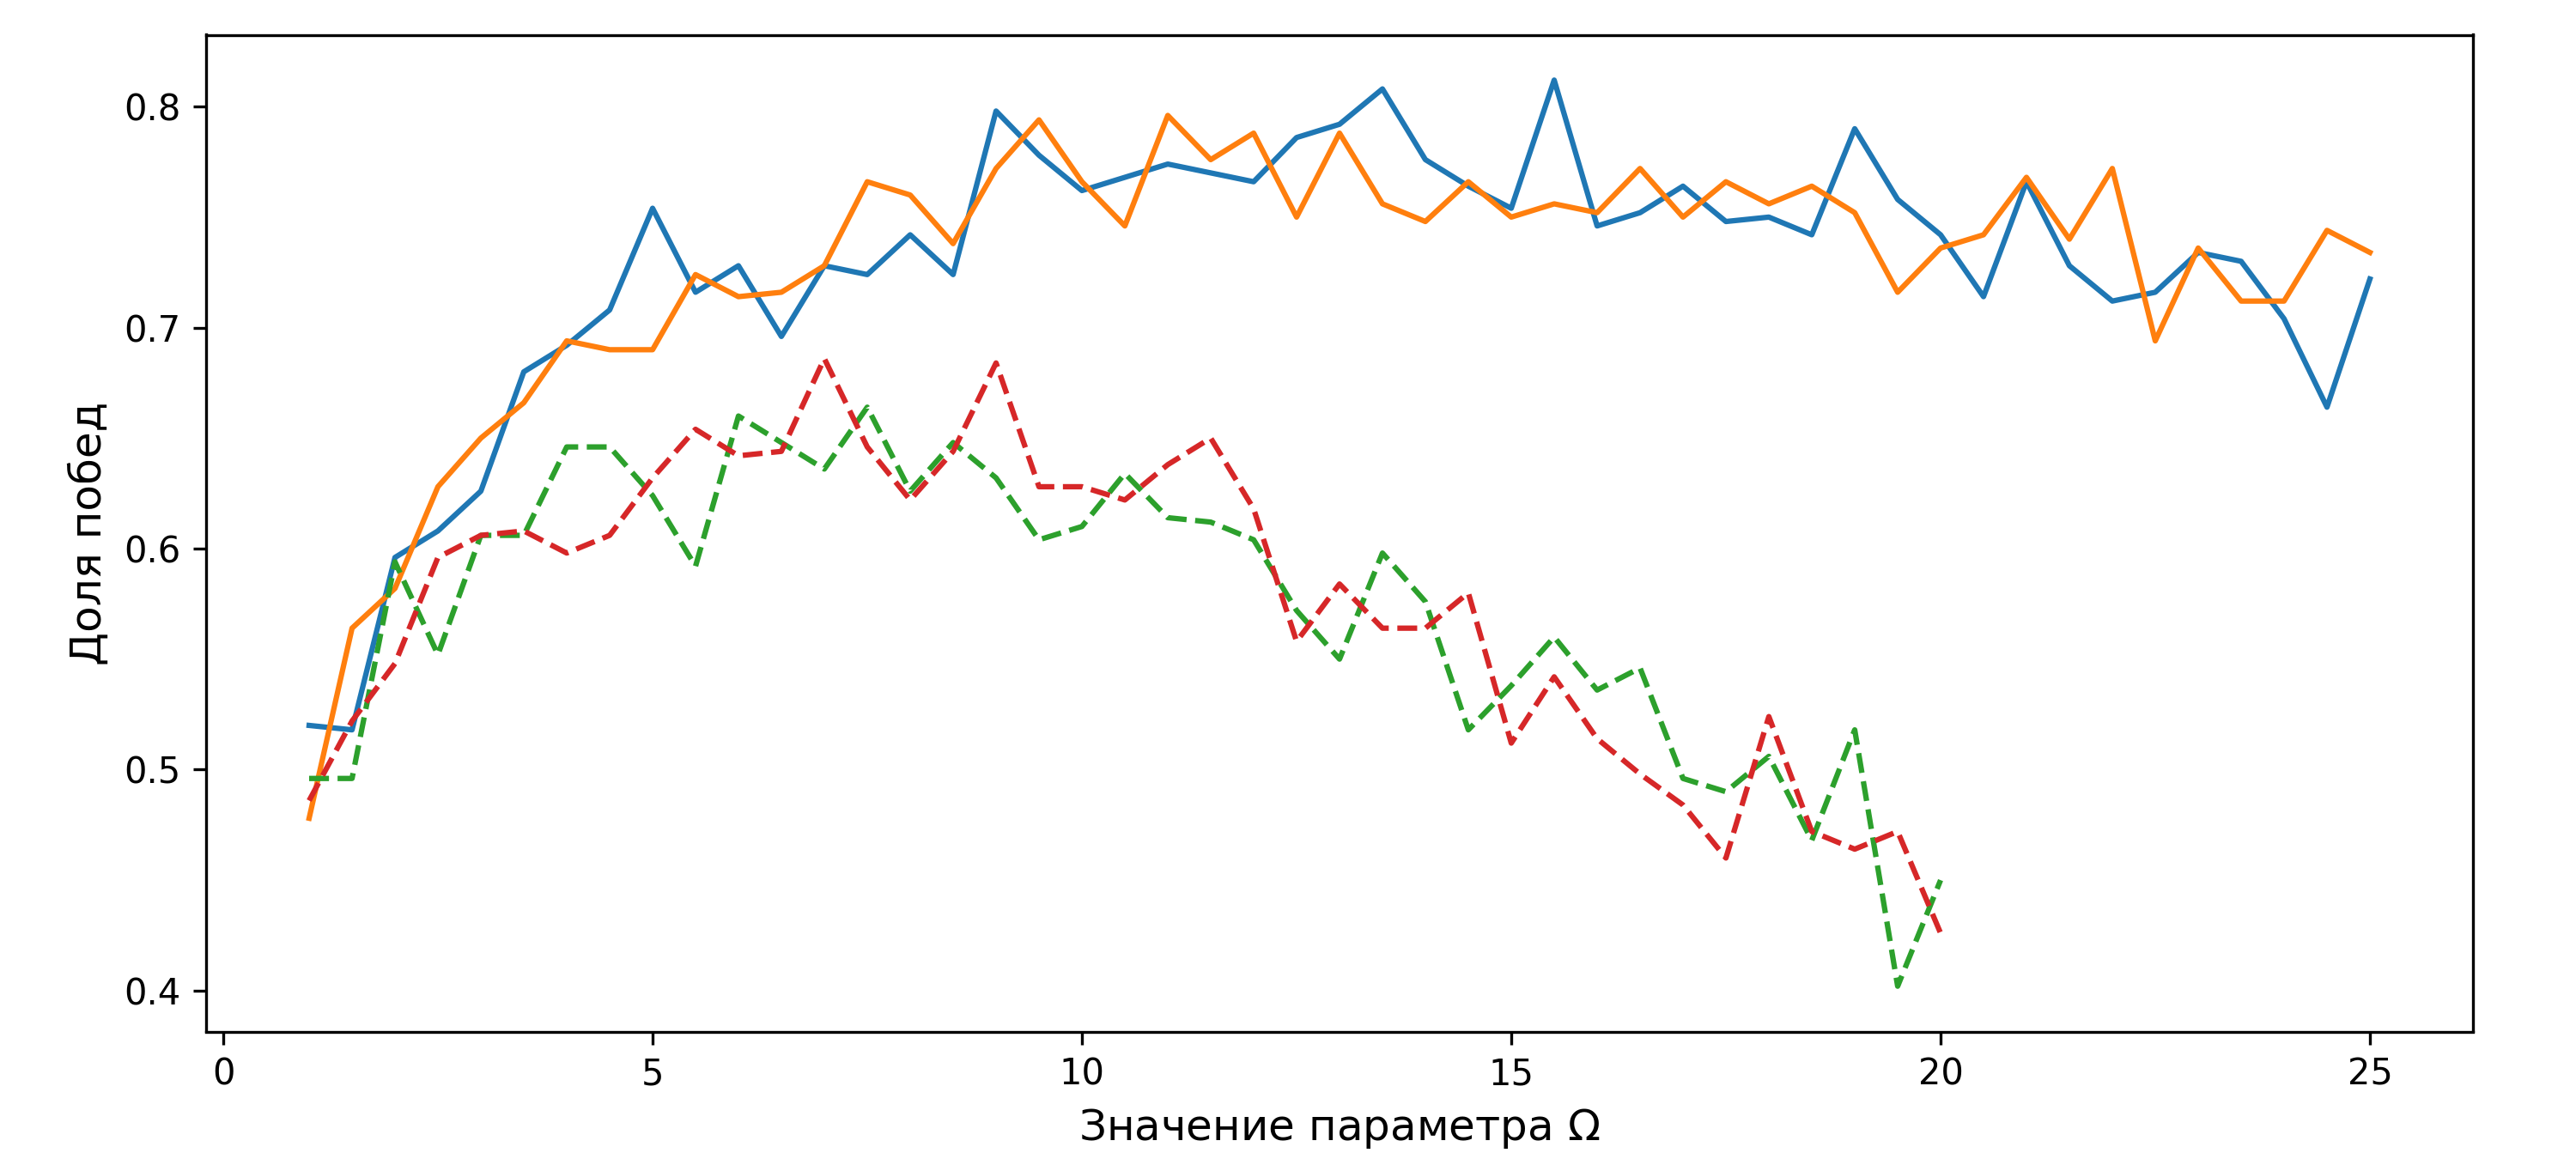
\includegraphics[width=\textwidth]{omega.png}
	\caption{Доля побед ААС в~зависимости от~параметра $\Omega$}\label{fig:aac_params}
\end{figure}

Результаты, приведённые в~таблице~\ref{table:highfreq}, показывают, что стратегия играет на~уровне ПС4. Но для~данной грамматики это вполне ожидаемый и хороший результат.

\begin{table}[!h]
	\small
	\setlength\tabcolsep{1.6pt}
	\centering
	\caption{Турнир (низкий шанс выпадения начальных продукций)}
	\label{table:lowfreq}
	\begin{tabular}{| c | c | c | c | c | c | c |}
		\hline
		      & СС         & УУСС      & ГСКС      & СКС        & ПС4        & AAC10     \\ \hline
		СС    & 250/238/12 & 199/297/4 & 185/313/2 & 268/232/0  & 153/341/6  & 91/405/4  \\ \hline
		УУСС  & 305/192/3  & 249/244/7 & 181/318/1 & 380/117/3  & 198/300/2  & 100/399/1 \\ \hline
		ГСКС  & 349/145/6  & 321/177/2 & 265/233/2 & 435/61/4   & 314/184/2  & 120/378/2 \\ \hline
		СКС   & 228/269/3  & 90/408/2  & 75/423/2  & 233/227/40 & 30/468/2   & 55/443/2  \\ \hline
		ПС4   & 352/141/7  & 286/209/5 & 200/298/2 & 460/39/1   & 244/244/12 & 89/410/1  \\ \hline
		AAC10 & 406/93/1   & 397/102/1 & 374/122/4 & 446/53/1   & 396/103/1  & 228/270/2 \\ \hline
	\end{tabular}
\end{table}
\sloppy
{
}
В~таблице~\ref{table:lowfreq} представлены фрагменты результатов турнира для~грамматики с~низким шансом выпадения начальных продукций. 

Выделяется явный фаворит в~лице адаптивной случайной стратегии. Она даже подходит на роль строго доминирующей стратегии.

Также выделяются плохие показатели стратегии коротких слов. Даже в партиях против~случайной стратегии она чаще проигрывает, чем побеждает. Причиной этого является та же проблема слишком быстрого получения сентенций. 

Снова довольно хорошо показывает себя глупая стратегия коротких слов, это происходит всё потому~же, из-за недостатка метрики~\ref{metric1}, который выражается в построении не самых коротких выводов. 

Можно отметить уменьшение отрыва переборной стратегии от~всех остальных. Это показывает ухудшение эффективности данной стратегии на грамматиках такого вида. Тем не менее, можно подчеркнуть, что при большой (или неограниченной) глубине перебора эта стратегия смогла бы показывать намного лучшие результаты.

По результатам рассмотрения смешанных стратегий, основанных на вероятностном выборе, можно сказать, что они не являются эффективными. Это вполне объяснимо, поскольку у нас имеется почти строго доминирующая стратегия. При смешивании такой стратегии с другими получается лишь ослабленная вариация изначально хорошей стратегии. Также это может быть связано с тем, что все стратегии, кроме адаптивной, направлены на~получение коротких выводов и~при их смешивании не получается строить более длинные выводы.

\section*{Сведения о финансировании}
Работа выполнена в рамках инициативной НИР ЯрГУ им. П.~Г.~Демидова № VIP-016.

\printbibliography

\end{document}

%%% Local Variables:
%%% mode: latex
%%% TeX-engine: luatex
%%% LaTeX-biblatex-use-Biber: t 
%%% TeX-master: t
%%% End:
